\chapter{Extending SuperBasic}\index{Extending SuperBasic}

\section{Introduction}
\label{ch7-intro}%\hyperlabel{ch7-intro}%

This time we are looking at extending SuperBasic by adding extra
    procedures and functions which can be loaded once after boot up and then
    used by any SuperBasic program that we load or type in afterwards.

Along the way, we will have to take a look at the manner in which we
    do the following:
\begin{itemize}[itemsep=0pt]

\item{}link assembler extensions (procedures and functions) into
        SuperBasic


\item{}fetching parameters


\item{}testing separators (eg the `\#' before a channel number
        etc)


\item{}the maths stack -{} and all its problems


\item{}returning values for functions


\item{}accessing the SuperBasic channel table

\end{itemize}

\section{Linking To SuperBasic}
\label{ch7-linking-superbasic}%\hyperlabel{ch7-linking-superbasic}%

When you have written some code that defines a new SuperBasic
    procedure or function, you must tell SuperBasic what it is called and
    where it lives. There is a vectored routine to do this and it is called
    \vector{BP\_INIT} (in QDOS) or \vector{SB\_INIPR} (in SMSQ). As an old hand at QDOS, I still
    use the QDOS definitions and names. As we are all using George Gwilt's
    \program{Gwasl}GWASL assembler, and it uses the QDOS names, we shall continue to do so in
    this series.

Start up the QED editor\program{QED Editor} (or your favourite) and type the following
    in:

\begin{lstlisting}[firstnumber=1,caption={Linking Extensions to SuperBasic},label={lst:LinkingSuperBasicExtensions}]
start   lea     define,a1       ; Pointer to the definition table
        move.w  BP_INIT,a2      ; The vector we need to use
        jmp     (a2)            ; Call the vectored routine
;                               ; and Return to SuperBasic
\end{lstlisting}

You will note that we only execute a small stub of code. This is
    simply because we are linking the new routines into SuperBasic and the
    actual code for the routines will be executed when a SuperBasic program
    uses one of the new routines. All will become clear.

The definition table required by \vector{BP\_INIT} has to be in the format shown in Table~\ref{tab:DefinitionBlockForBPINIT} and it must start at an even address. A1.L points at the table when
    \vector{BP\_INIT} is called:

\begin{table}[htbp]
\centering
\begin{tabular}{l l}  % Set this correctly ...
\toprule
\textbf{Size} & \textbf{Purpose} \\
\midrule
%
word & How many new procedures (A1 points here)\\
\multicolumn{2}{c}{Repeat for each procedure:} \\
word  & Offset to code start for this procedure\\
byte  & How many bytes in the procedure name\\
bytes & The procedure name\\
word  & Zero = end of procedures\\
word  & How many new functions\\
\multicolumn{2}{c}{Repeat for each function:}\\
word  & Offset to code start for this function\\
byte  & How many bytes in the function name\\
bytes & The function name\\
word  & Zero = end of functions \& table\\
%
\bottomrule
\end{tabular}
\caption{Definition Block For BP\_INIT}
\label{tab:DefinitionBlockForBPINIT}
\end{table}

As an example, our code file will introduce 1 new procedure and the
    definition table will be set up like the following which you should now
    type into the editor following on from the code that is already there
   :

\begin{lstlisting}[firstnumber=1,caption={Example Extension Parameter Table},label={lst:ExampleParameterTable}]
define  dc.w    1               ; 1 new procedure
        dc.w    psi_cls-*
        dc.b    7,'PSI_CLS'
        dc.w    0               ; End of procedures

        dc.w    0               ; Number of functions
        dc.w    0               ; End of functions
\end{lstlisting}

Notice that the format of the procedure name is slightly different
    from normal QDOS string in that the size of the name is stored in a \emph{byte}
    and not in a word.

Now then, there is a caveat -{} isn't there always? If the average
    length of the names of all the procedures, or functions, is greater than 7
    then the simple word for the number of procedures or functions is changed
    to the value given by this calculation:

$(\text{total number of characters in proc names} + \text{number of procedures} + 7) / 8$

Checking our table above we have a total of 7 characters in the
    procedure name and there is 1 new procedure. This gives an average of 7
    characters per name (round up always!) so we are ok.

And that is it. On QL's of JM vintage and below, the machine must be
    NEW'd before you can use them. On JS and above, this need not be
    done.

Once a set of procedures and/or functions has been linked into
    SuperBasic, the definition block is no longer required. If your code
    requires the use of some workspace, then you can use the definition table.
    Just make sure that you don't use more bytes that there are available
   !

So, let's write our first procedure.

\section{Procedures}
\label{ch7-procedures}%\hyperlabel{ch7-procedures}%

Procedures in assembly are very much like PROCedures in SuperBasic.
    For example, consider the following:\program{PSI\_CLS}

\begin{lstlisting}[firstnumber=1,language={}]
1000 DEFine PROCedure PSI_CLS(chan%, P%, S%, I%)
1010   PAPER #chan%, P%
1020   STRIP #chan%, S%
1030   INK #chan%, I%
1040   CLS #chan%
1050 END DEFine PSI_CLS
\end{lstlisting}

This simple routine is probably at the heart of many SuperBasic
    programs and is called like this:

\begin{lstlisting}[firstnumber=1,]
100 PSI_CLS 1, 2, 4, 0
\end{lstlisting}

To give channel \#1 red paper, green strip and black ink. Assembler
    procedures are very similar and in fact we shall now dive straight in and
    convert the above into assembler.

Back into the QED editor\program{QED Editor} with the code from the start of this
    article typed in. We have so far typed the code to link the new procedure
    and the definition block for the new procedure, now we need to write the
    code for the procedure itself. Your file should look like this so far
   :

\begin{lstlisting}[firstnumber=1,caption={PSI\_CLS Definition Table},label={lst:PsiClsDefinitionTable}]
start   lea     define,a1       ; Pointer to the definition table
        move.w  BP_INIT,a2      ; The vector we need to use
        jsr     (a2)            ; Call the vectored routine
        rts                     ; Return to SuperBasic

define  dc.w    1               ; 1 new procedure
        dc.w    psi_cls-*
        dc.b    7,'PSI_CLS'
        dc.w    0               ; End of procedures

        dc.w    0               ; Number of functions
        dc.w    0               ; End of functions
\end{lstlisting}

In the definition table there is an offset word to the start address
    of the new procedure. Ours is defined like this:

\begin{lstlisting}[firstnumber=1,]
        dc.w    psi_cls-*
\end{lstlisting}

Which is a useful way to get the assembler to calculate the offset
    for us. The `*' is assembler short-{}hand for `where I am now' or `the
    current address'. Our example uses the label psi\_cls so our code has to
    start there.

On with the procedure. In assembler you must take great care to
    ensure that you have enough parameters etc (see below) and that they are
    all the correct type. In this example, we will get using integer
    parameters but the first one must have a hash (\#) in front of it. Of
    course, when using INK, PAPER etc in SuperBasic, you can default the
    channel number and \#1 will be used instead. This means that the following
    statements are equivalent:

\begin{lstlisting}[firstnumber=1,]
2000 PAPER #1,2
2010 PAPER 2
\end{lstlisting}

It would be nice if our PSI\_CLS\program{PSI\_CLS} routine did a similar thing so that
    the following was equivalent:

\begin{lstlisting}[firstnumber=1,]
2500 PSI_CLS #1, 2, 2, 0
2510 PSI_CLS 2, 2, 0
\end{lstlisting}

This turns out to be quite easy to do.

Here then, is a list of what our procedure must do:
\begin{itemize}[itemsep=0pt]

\item{}Count how many parameters were supplied. There must be 3 or
        4.


\item{}If 4 parameters supplied, check that the first parameter has a
        hash in front of it.


\item{}Fetches all parameters onto the maths stack.


\item{}Convert parameters from maths stack to registers \& validates
        them.


\item{}Set the paper, strip and ink colours for the correct channel,
        defaulting to \#1 as appropriate, if only 3 parameters were
        supplied.


\item{}Clear the channel using CLS.


\item{}Returns to SuperBasic.


\item{}Abort nicely whenever it detects an error.

\end{itemize}

Type the following after the definition block:
\program{PSI\_CLS}
\begin{lstlisting}[firstnumber=13,caption={PSI\_CLS - The Final Version - Part 1},label={lst:PsiClsFinalVersionPart1}]
err_bp      equ     -15            ; Bad parameter error
err_no      equ     -6             ; Channel not open
bv_chbas    equ     $30            ; Offset to channel table
bv_chp      equ     $34            ; Offset to channel table end
bv_rip      equ     $58            ; Maths stack pointer

psi_cls     move.l  a5,d7          ; End of parameters
            sub.l   a3,d7          ; Minus start of parameters
            divu    #8,d7          ; How many parameters?
            cmpi.w  #3,d7          ; Defaulting channel id?
            beq.s   hash_ok        ; yes, skip hash check

*----------------------------------------------------------------
* We do not have 3 parameters so test for 4 and if not found, 
* error exit. If we do have 4 then the first must have a hash in
* front.
*----------------------------------------------------------------
hash_check  cmpi.w  #4,d7          ; We need  4 parameters
            bne.s   error_bp       ; Oops!
            btst    #7,1(a6,a3.l)  ; Is there a # before p1?
            beq.s   error_bp       ; No, we reject it then

hash_ok     move.w  ca_gtint,a2    ; We want word integers
            jsr     (a2)           ; Fetch them all
            tst.l   d0             ; Did it work?
            beq.s   got_ok         ; Yes it did
            rts                    ; Bale out otherwise

*----------------------------------------------------------------
* We expected to get 3 or 4 parameters and should have, but now 
* that we have got them, check to make sure we have received that 
* which we expected to.
*----------------------------------------------------------------
got_ok      cmpi.w  #4,d3          ; Were there 4 of them?
            beq.s   got_4          ; Yes

            cmpi.w  #3,d3          ; Maybe default channel in use
            beq.s   got_3          ; So that is ok too

error_bp    moveq   #err_bp,d0     ; Bad Parameter error code
error_exit  rts                    ; Bale out with error

*----------------------------------------------------------------
* We have 4 parameters, so fetch the channel id into D0 - this is
* the first of the parameters. We need to tidy the maths stack as 
* well so that get_rest works correctly regardless of whether we 
* have 3 or 4 parameters.
*----------------------------------------------------------------
got_4       move.w  0(a6,a1.l),d0   ; Get channel id
            bmi.s   error_bp       ; We don't like -ve channels
            adda.l  #2,a1          ; Tidy stack pointer
            bra.s   get_rest       ; Skip default channel id bit


*----------------------------------------------------------------
* At this point we default the channel being used to #1. By
* moving one to D0 and processing as normal, we can do this 
* without much effort.
*----------------------------------------------------------------
got_3       moveq   #1,d0          ; Default channel is #1

*----------------------------------------------------------------
* Here convert the SuperBasic channel number in D0 into an 
* internal id in A0 and bale out if it fails, or if the channel
* is not open or has been closed - there is a difference. 
* A closed channel has a negative id while a channel not yet 
* opened is not in the table.
*----------------------------------------------------------------
get_rest    bsr     channel_id     ; Convert DO->QDOS id in A0.L
            bne.s   error_exit     ; Bale out if errors
\end{lstlisting}

At this point we have (A6,A1) pointing to the paper parameter on the
    stack and A0.L holding the channel id for the requested channel (or the
    default of \#1). Now we can set the paper colour (which does not set the
    strip like SuperBasic does!)

Looking at the QDOS documentation for SD\_SETPA and the others, we
    see that A1 is `undefined' on return from the routine. This is bad so we
    need to preserve it across calls or we can fetch all the parameters first.
    Registers D4 to D7 are not mentioned in the documentation so they are
    preserved/not used by the routines so we shall fetch the parameters into
    these registers first of all and this way we can also validate them for
    errors.

\begin{lstlisting}[firstnumber=last,caption={PSI\_CLS - The Final Version - Part 2},label={lst:PsiClsFinalVersionPart2}]
*----------------------------------------------------------------
* Because we tidied the stack pointer in A1 when we fetched the 
* channel id, the following code expects to see the paper colour 
* at 0(A6,A1) and this is the same as if we never were supplied 
* with a channel id in the first place - cunning stuff eh?
*
* Fetch the remaining 3 parameters into registers that will not 
* be trashed by the QDOS routines that set the paper, strip and
* ink. We reject any parameter which is negative as we don't deal
* with negative colours and just in case, we also mask out the 
* high work of the parameter to ensure it is in range 0 to 255.
*
* NOTE: we could do away with the negative check and just mask. 
* This would in effect convert from a negative to a positive 
* number - but this is the real world (?) and we have to perform
* parameter validation.
*----------------------------------------------------------------
            move.w  0(a6,a1.l),d4  ; Paper in D4
            bmi.s   error_bp       ; Negative is bad news
            andi.w  #$00ff,d4      ; Force range 0 - 255

            move.w  2(a6,a1.l),d5  ; Strip in D5
            bmi.s   error_bp       ; Negative is bad news
            andi.w  #$00ff,d5      ; Force range 0 - 255

            move.w  4(a6,a1.l),d6  ; Ink in D6
            bmi.s   error_bp       ; Negative is bad news
            andi.w  #$00ff,d6      ; Force range 0 - 255

            adda.l  #6,a1          ; Tidy the stack

            moveq   #sd_setpa,d0   ; Paper trap code
            move.w  d4,d1          ; Paper colour
            moveq   #-1,d3         ; Infinite timeout
*                                  ; Channel id is still in A0
            trap    #3             ; Set the paper
            tst.l   d0             ; OK?
            bne.s   error_exit     ; No bale out

*----------------------------------------------------------------
* Now the paper has been set, and the documentation says that A0
* is preserved along with D3, we can set the strip colour now.
*----------------------------------------------------------------
            moveq   #sd_setst,d0   ; Strip trap code
            move.w  d5,d1          ; Strip colour
            trap    #3             ; Set the strip
            tst.l   d0             ; OK?
            bne.s   error_exit     ; No bale out

*----------------------------------------------------------------
* Now the strip has been set, and the documentation says that A0
* is preserved along with D3, we can set the ink colour now.
*----------------------------------------------------------------
            moveq   #sd_setin,d0   ; Ink trap code
            move.w  d6,d1          ; Ink colour
            trap    #3             ; Set the Ink
            tst.l   d0             ; Ok?
            bne.s   error_exit     ; No bale out

*----------------------------------------------------------------
* And finally, we can CLS the screen. 
*----------------------------------------------------------------
            moveq   #sd_clear,d0   ; CLS whole screen
            trap    #3             ; Do it
            bra.s   error_exit     ; All done


*----------------------------------------------------------------
* This routine takes a SuperBasic channel number in D0 and 
* converts it into a QDOS internal channel id in A0. If the 
* channel is closed or not yet opened, the routine returns D0 = 
* ERR_NO and A0 is invalid. 
* D0 will be zero if all is ok.
*----------------------------------------------------------------
channel_id  mulu    #$28,d0         ; Offset into channel table
            add.l   bv_chbas(a6),d0 ; Add table start address
            cmp.l   bv_chp(a6),d0  ; Valid?
            bge.s   ch_bad         ; No, channel # off end
            move.l  0(a6,d0.l),d0  ; Channel id
            bmi.s   ch_bad         ; Channel closed
            move.l  d0,a0          ; We need id in A0
            moveq   #0,d0          ; No errors
            rts                    ; Finished

ch_bad      moveq   #err_no,d0     ; Channel not open (-6)
            rts                    ; Bale out
\end{lstlisting}

Save the file and assemble it using GWASL\program{Gwasl}. Once all errors have been
    sorted out, either LRESPR it or ALCHP/LBYTES/CALL in the normal manner. If
    you have a JM and below, type NEW then try this:

\begin{lstlisting}[firstnumber=1,]
PSI_CLS #1, 2, 4, 0  (or PSI_CLS 2, 4, 0)
\end{lstlisting}

And see what happens when you

\begin{lstlisting}[firstnumber=1,]
PRINT 'Hello world' (or PRINT #1, 'Hello world')
\end{lstlisting}

If you have a JS or above, then just try it without the NEW.

You should see the words `Hello world' written in black, on a green
    strip on red paper -{} assuming your display can handle the colour mixture
   !

In the code, you will notice that whenever I detect an error, I
    simply return to SuperBasic with the error code in D0. This doesn't look
    very friendly does it? Actually, QDOS is very friendly when it comes to
    procedures because in the event of an error, QDOS will do all the tidying
    up that we need to do so we don't have to worry about it. This is
    discussed below in Section~\ref{ch7-functions}~\nameref{ch7-functions} and in Section~\ref{ch7-maths-stack}~\nameref{ch7-maths-stack}.

\section{Functions}
\label{ch7-functions}%\hyperlabel{ch7-functions}%

Wouldn't it be nice to do this instead of the above:

\begin{lstlisting}[firstnumber=1,]
PSI_CLS #1, RED, GREEN, BLACK
\end{lstlisting}

In SuperBasic this would be done either by:

\begin{lstlisting}[firstnumber=1,]
DEFine FuNction RED
    return 2
END DEFine RED

DEFine FuNction GREEN
    return 4
END DEFine GREEN

DEFine FuNction BLACK
    return 0
END DEFine BLACK
\end{lstlisting}

OK, I know it could be done like this:

\begin{lstlisting}[firstnumber=1,]
RED = 2
GREEN = 4
BLACK = 0
\end{lstlisting}

but we are dealing with machine code functions and this is more
    illustrative of what we are about to do. (So there!)

We shall now extend our original example so that we can specify
    colour values by name -{} this is much more friendly in my opinion.

The following two lines in the definition block need to be removed
   :

\begin{lstlisting}[firstnumber=1,caption={Colour Functions},label={lst:ColourFunctions}]
        dc.w    0               ; Number of functions
        dc.w    0               ; End of functions
\end{lstlisting}

And replaced by the following:

\begin{lstlisting}[firstnumber=1,caption={Colour Functions},label={lst:ColourFunctions}]
        dc.w    8               ; There are 8 functions

        dc.w    black-*         ; First function
        dc.b    5,'BLACK'

        dc.w    blue-*          ; Second function
        dc.b    4,'BLUE'

        dc.w    red-*           ; Third function
        dc.b    3,'RED'

        dc.w    cyan-*          ; Fourth function
        dc.b    4,'CYAN'

        dc.w    green-*         ; Fifth function
        dc.b    5,'GREEN'

        dc.w    magenta-*       ; Sixth function
        dc.b    7,'MAGENTA'

        dc.w    yellow-*        ; Seventh function
        dc.b    6,'YELLOW'

        dc.w    white-*         ; Eighth function
        dc.b    5,'WHITE'

        dc.w    0               ; End of functions
\end{lstlisting}

The following is the code for the new functions, type it into the
    file after the end of the `channel\_id' subroutine:

\begin{lstlisting}[firstnumber=1,]
black       moveq   #0,d7
            bra.s   return_d7

blue        moveq   #1,d7
            bra.s   return_d7

red         moveq   #2,d7
            bra.s   return_d7

magenta     moveq   #3,d7
            bra.s   return_d7

green       moveq   #4,d7
            bra.s   return_d7

cyan        moveq   #5,d7
            bra.s   return_d7

yellow      moveq   #6,d7
            bra.s   return_d7

white       moveq   #7,d7

*----------------------------------------------------------------
* This routine returns the word value in d7 to SuperBasic as the 
* result of the function we are running. It requires two bytes on
* the top of the maths stack and because there were no parameters
* supplied to any of the functions, I can safely ask QDOS for 
* these two bytes.
*----------------------------------------------------------------
return_d7   move.l  bv_rip(a6),a1   ; Because we had no params
            moveq   #2,d1           ; Two bytes required
            move.w  bv_chrix,a2     ; Allocate maths stack space
            jsr     (a2)            ; Go get some space.
*                                   ; No errors are returned.

*----------------------------------------------------------------
* The maths stack has been extended by two bytes BUT it may have
*  moved around in memory so we need to get the stack pointer 
* into A1 again.
*----------------------------------------------------------------
            move.l  bv_rip(a6),a1   ; New top of stack
            subq.l  #2,a1           ; Space for our result
            move.w  d7,0(a6,a1.l)   ; Stack the result
            move.w  #3,d4           ; Signal word result on stack
            move.l  a1,bv_rip(a6)   ; Store new top of stack
            clr.l   d0              ; No errors
            rts                     ; Return result to SuperBasic
\end{lstlisting}

That is the end of the code. Assemble it, debug it and test it using
    the following:

\begin{lstlisting}[firstnumber=1,]
PAPER GREEN
STRIP RED
INK BLACK
CLS
PRINT "Hello world"
\end{lstlisting}

or, if you like:

\begin{lstlisting}[firstnumber=1,]
PSI_CLS GREEN, RED, BLACK
PRINT "Hello world"
\end{lstlisting}

In the procedure, PSI\_CLS\program{PSI\_CLS}, we obtained some parameters for the
    various colours and channels. I shall now discuss how this is done in much
    more detail.

\section{Getting Parameters}\index{Fetching Parameters}
\label{ch7-parameters}%\hyperlabel{ch7-parameters}%

On entry to a machine code extension (ie not an EXEC'd job or a
    CALLed routine) certain registers are set up with very useful values.
    These are shown in Table~\ref{tab:RegsitserSettingsOnEntryToSuperBasicExtensions}.
    
\begin{table}[htbp]
\centering
\begin{tabular}{l l}  % Set this correctly ...
\toprule
\textbf{Register} & \textbf{Value} \\
\midrule
%
A1 & \emph{Allegedly} points to the top of the maths stack relative to A6, however, see below.\\
A3 & Points to the start of the name table entry for the first parameter.\\
A5 & Points to the first byte \emph{after} the name table entry for the last parameter.\\
A6 & Base address of SuperBasic. Do not change this register.\\
%
\bottomrule
\end{tabular}
\caption{Register Settings On Entry To SuperBasic Extensions.}
\label{tab:RegsitserSettingsOnEntryToSuperBasicExtensions}
\end{table}

A1 is supposed to point at the top of the maths stack (see below)
    relative to A6, but I have found out the hard way that this is only the
    case when the procedure or function being executed has some parameters and
    they have been fetched. A1 is set to the amount of space used (or free) on
    the maths stack on entry to a procedure. (See Maths Stack below for full
    details.)

A3 points at the address of the first byte of the first entry in the
    name table\index{Name Table} for this procedure or function. Again, this is relative to
    A6.

A5 points at the address of the first byte \emph{after} the last name table
    entry for this procedure or function. Again this is relative to A6.

A6 should never be changed as it points to the base of the
    SuperBasic job and almost all the various routines involving the maths
    stack and getting/returning parameters rely on addresses being relative to
    A6.

So we can now check to see how many parameters we have by the
    following calculation:

$(A5-A3)/8$

There are 8 bytes in each name table entry. Full details of the name
    table entries are given below.

If we have 3 parameters, then the name table entries will look like
     \figurename~\ref{fig:NameTableEntriesForThreeParameters}:\index{Name Table}

\begin{figure}[h]
\center
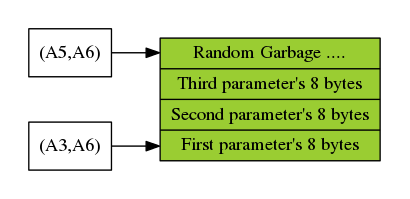
\includegraphics[width=0.5\textwidth]{Content/images/Name_Table_Entries.png}
\caption{Name Table Entries for Three Parameters.}
\label{fig:NameTableEntriesForThreeParameters}
\end{figure}

So (A3,A6) points to the first byte of the first parameter and is
    the lowest address, (A5,A6) points to the first byte past the last
    parameter and is the highest address.

The first name table entry starts at 0(A3,A6) and ends at 7(A3,A6).
    The second starts at 8(A3,A6) and ends at 15(A3,A6) and the last starts at
    16(A3,A6) and stops at 23(A3,A6).

When fetching parameters from the name list onto the maths stack, we
    can use some vectored utilities to get them for us. These allow the
    retrieval of strings, long words, integers (short words) and floating
    point values. They all expect A3 and A5 to be set up correctly as above.
    A3 and A5 are trashed by the routines, so if you have to check any
    parameter separators etc, then you must do it before calling the fetch
    routines.

When the routines return, they set D3.W to the number of parameters
    fetched and set A1 to the correct value for the top of the maths stack -{}
    relative to A6 of course. Now we can access the values of each parameter
    separately as we like. On return the first parameter in the list is stored
    at 0(A1,A6), the next is above the first and so on. When fetching
    parameters p1, p2, p3 from a procedure or function call, they will end up
    on the maths stack in the correct order -{} 0(A1,A6) will be pointing at p1
    on the stack.

The parameter fetching routines are listed in Table~\ref{tab:VectoredRoutinesForParameterFetching}.
\begin{table}[htbp]
\centering
\begin{tabular}{l l}  % Set this correctly ...
\toprule
\textbf{Vector} & \textbf{Purpose} \\
\midrule
%
\vector{CA\_GTINT} & fetch integer parameters (2 bytes each).\\
\vector{CA\_GTLIN} & fetch long parameters (4 bytes each).\\
\vector{CA\_GTFP} & fetch floating point parameters (6 bytes each).\\
\vector{CA\_GTSTR} & fetch string parameters (variable length).\\
%
\bottomrule
\end{tabular}
\caption{Vectored Routines For Parameter Fetching.}
\label{tab:VectoredRoutinesForParameterFetching}
\end{table}


They require to be called as follows:

\begin{lstlisting}[firstnumber=1,caption={Using the Vectored Parameter Fetching Utilities},label={lst:ParameterFetchingUtilities}]
start   move.w  ca_gtint,a2     ; Fetch all params as word ints
        jsr     (a2)            ; Do it
        tst.l   d0              ; Did it work?
        beq.s   ok              ; Yes
        rts                     ; Return to SuperBasic

ok      ...                     ; carry on here
\end{lstlisting}

At this point, D3.W can be tested to check that the correct number
    of parameters has been fetched.

\begin{lstlisting}[firstnumber=1,caption={Checking Parameter Counts},label={lst:CheckingParameterCounts}]
start   cmpi.w  #4,d3           ; Were there 4 parameters?
        beq.s   ok_4            ; Yes
        moveq   #-15,d0         ; Bad parameter error code = -15
        rts                     ; and back to SuperBasic

ok_4    ...                     ; Carry on here
\end{lstlisting}

To access the parameters we need to get the data off of the maths
    stack and into our working registers, as follows:

\begin{lstlisting}[firstnumber=1,caption={Fetching Parameter Values},label={lst:FetchingParameterValues}]
        move.w  0(a6,a1.l),d1   ; Parameter one
        move.w  2(a6,a1.l),d2   ; Parameter two
        move.w  4(a6,a1.l),d3   ; Parameter three
        move.w  6(a6,a1.l),d4   ; Parameter four
\end{lstlisting}

and so on. Now that we have our parameters, we need do nothing more
    with the maths stack if we are inside the code of a procedure. If we are
    in a function then we \emph{must} tidy the maths stack. This is simply done by
    adding the size of all parameters on the stack to A1. In our example we
    have 4 word length parameters, so we should add 8 to A1 as follows
   :

\begin{lstlisting}[firstnumber=1,]
        adda.l  #8,a1           ; Reset maths stack
\end{lstlisting}

As mentioned, there is no need to do this in a procedure, but if you
    have to learn to do it for a function, you are as well to learn to do it
    for everything -{} that way you don't forget to do it and cause a hanging
    QL.

Tidying a stack with strings on is more difficult and it is probably
    best done as each one is removed. For example, say we have two strings on
    the stack after a call to \vector{CA\_GTSTR} then we get them off as follows
   :
\index{Tidying the Maths Stack}
\begin{lstlisting}[firstnumber=1,caption={Tidying a String from the Maths Stack - Part 1},label={lst:StringStackTidyPart1}]
    cmpi.w  #2,d3           ; Were there two strings?
    beq.s   ok              ; Yes
    moveq   #-15,d0         ; Bad parameter
    rts                     ; Exit to SuperBasic

ok  lea     buffer_a,a2     ; Destination for one string
    lea     0(a6,a1.l),a3   ; Source for string
    bsr     copy_str        ; Copy
    move.w  0(a6,a1.l),d0   ; Size word
    addq.w  #3,d0           ; Make bigger
    bclr    #0,d0           ; Make even
    add.w   d0,a1           ; This will sign extend remember!
\end{lstlisting}

Ok, so we added the size of the first string plus 2 for the size of
    the size word as well, to A1 having made it even so the stack is now
    cleared of the first string. This leaves one string with its size word
    sitting at 0(A6,a1.l) ready for the next copy:

\begin{lstlisting}[firstnumber=1,caption={Tidying a String from the Maths Stack - Part 2},label={lst:StringStackTidyParty2}]
    lea     buffer_b,a2     ; Destination for next string
    lea     0(a6,a1.l),a3   ; Source for string
    bsr     copy_str        ; Do the copy
    move.w  0(a6,a1.l),d0   ; Size word
    addq.w  #3,d0           ; Make bigger
    bclr    #0,d0           ; Make even
    add.w   d0,a1           ; This will sign extend too!
\end{lstlisting}

and there you have a tidy stack once again.

You could ask `if we have to restore A1 to its value on entry, why
    not just save A1 and then restore it afterward?'. Like this:

\begin{lstlisting}[firstnumber=1,caption={How to Hang the QL},label={lst:HowToHangTheQL}]
start   move.l  bv_rip(a6),a1   ; Fetch top of Maths Stack
        move.l  a1,-(a7)        ; Stack it for later

        ; Do lots of stuff here - fetching parameters etc

        move.l  (a7)+,a1        ; Restore A1

        ; and so on
\end{lstlisting}

Well, you could, but at certain times there will be a hung QL and
    you will not know why. The reason is simple, but difficult to find or
    trace. When you fetch parameters onto the maths stack, it can \emph{move around in memory}. Preserving the original value is fine if the stack stays put, but
    if it moves and you set BV\_RIP to the old value, you can get into all
    sorts of trouble. It is best to keep the stack tidy using the methods
    described above.

\subsection{Keeping Things Even}
\label{ch7-keep-things-even}%\hyperlabel{ch7-keep-things-even}%

You may well also ask ``What is all this add 3 and clear bit 0
      nonsense then?'' Think about it in binary for a bit. We have the word
      size of the string in D0.W and we must ensure that we add an even number
      of bytes to A1. We must also remember to add 2 to A1 for the size of the
      size word itself.

Lets try this with an even number first of all. Even numbers are
      detected by bit zero being clear, so:
\begin{table}[htbp]
\centering
\begin{tabular}{c c c}  % Set this correctly ...
\toprule
\textbf{D0} & \textbf{D0 + 3} & \textbf{Result} \\
\midrule
%
2 & 5 & 4\\
4 & 7 & 6\\
10 & 13 & 12\\
%
\bottomrule
\end{tabular}
\caption{Keeping even numbers even.}
\label{tab:KeepingEvenNumbersEven}
\end{table}

So you can see what is happening. D0 always ends up being D0 + 2
      and is always even. This is good as it is what we want. What about odd
      numbers then?

\begin{table}[htbp]
\centering
\begin{tabular}{c c c}  % Set this correctly ...
\toprule
\textbf{D0} & \textbf{D0 + 3} & \textbf{Result} \\
\midrule
%
3 & 6 & 6\\
5 & 8 & 8\\
11 & 14 & 14\\
%
\bottomrule
\end{tabular}
\caption{Keeping odd numbers even.}
\label{tab:KeepingOddNumbersEven}
\end{table}


So is this good then? Remember that the maths stack must be kept
      even. When odd length strings are copied onto it by \vector{CA\_GTSTR} it pads out
      the space on the stack with a rubbish byte (CHR\$(0) to be precise) which
      is never used. The size word remains odd.

So for an odd sized string we need to add 2 for the size word, the
      odd number of bytes and one spare for the padding. Our 3 lines of code
      handle this for all cases -{} even or odd sized strings. The code is good!

Of course it would be simple to do this:

\begin{lstlisting}[firstnumber=1,caption={Long Way to Keep Things Even},label={lst:LonegWayToKeepThingsEven}]
        move.w  0(a6,a1.l),d0   ; Size word
        btst    #0,d0           ; Is it even?
        beq.s   even            ; Yes
        addq.w  #1,d0           ; Add 1 for padding byte

even    addq.w  #2,d0           ; Add 2 ro the size word
        add.w   d0,a1           ; And add with sign extension
\end{lstlisting}

But this is extra typing and takes longer, so the simple case
      shown above, works all the time.

\subsection{Two Of These And One Of Those Please}\index{Fetching mixed type parameters}
\label{ch7-mixed-parameters}%\hyperlabel{ch7-mixed-parameters}%

What do you do if you want to get hold of two long words and a
      string?

Let us assume that you are writing an extension procedure that has this
      format:

\begin{lstlisting}[firstnumber=1,]
DO_SOMETHING long_1, long_2, string_1
\end{lstlisting}

This has two different types of parameters and we cannot fetch
      them all in one go unless we can read the long parameters as strings and
      convert them ourselves. It is quite easy to fetch these parameters -{} you
      just do it in two goes.

In the code we know that A3 and A5 hold the start and stop
      addresses of the parameters in the Name Table. If we set A5 to be A3 +
      16 and then collect long words we will get our two long words. We can
      then set A5 back to its original value and set A3 to this less 8 and
      fetch the final parameter as a string. Here we go then:

\begin{lstlisting}[firstnumber=1,caption={Fetching Mixed Type Parameters},label={lst:FetchingMixedTypeParameters}]
get_longs   move.l  a5,-(a7)        ; Save last parameter pointer
            lea     16(a3),a5       ; Set A5 for two parameters
            move.w  ca_gtlint,a2    ; Fetch all (2) longs
            jsr     (a2)            ; Do it
            tst.l   d0              ; OK?
            beq.s   got_long        ; Yes
            rts                     ; Exit with error code

got_long    cmpi.w  #2,d3           ; Were there two?
            bne.s   bad_params      ; No, bale out
            move.l  (a7)+,a5        ; A5 holds address of p3
            lea     -8(a5),a3       ; There can be only one!
            move.w  ca_gtstr,a2     ; Fetch as strings now
            jsr     (a2)            ; Do it
            tst.l   d0              ; OK?
            beq.s   got_string      ; Yes
            rts                     ; Exit with error code

bad_params  moveq   #-15,d0         ; Bad parameter error
            rts                     ; Exit to SuperBasic

got_string  ; continue from here
\end{lstlisting}

Ok, so now what does the maths stack look like? Remember when
      fetching parameters they end up on the stack in the order you want them
      with the first at the lowest address and the next above it and so on.
      This time, we fetched two longs and a string in two different calls.
      This means that after the first fetch the maths stack looks like  	    \figurename~\ref{fig:MathsStackAfterTwoLongInts}:

\begin{figure}[h]
\center
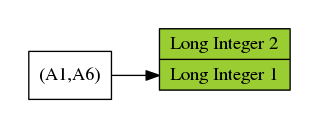
\includegraphics[width=0.5\textwidth]{Content/images/Maths_Stack_2_Long.png}
\caption{Maths Stack After Fetching Two Long Integer Parameters.}
\label{fig:MathsStackAfterTwoLongInts}
\end{figure}

But then we fetched a string and it got put onto the maths stack
      so it now looks like \figurename~\ref{fig:MathsStackAfterTwoLongIntsPlusString}:

\begin{figure}[h]
\center
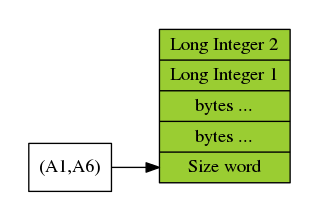
\includegraphics[width=0.5\textwidth]{Content/images/Maths_Stack_2_Long_and_String.png}
\caption{Previous Maths Stack After Fetching a String Parameter.}
\label{fig:MathsStackAfterTwoLongIntsPlusString}
\end{figure}

QDOS is very helpful here. If during the course of fetching the
      string, the maths stack had to be moved in memory, QDOS will preserve
      the current contents so that `long\_1' and `long\_2' will still be there
      when you come around to using their values. Nice!

In this discussion we mentioned the name table. This is discussed
      in detail next. Do you get the feeling that this chapter is written upside down?

\section{Name Table Entries}\index{Name Table}
\label{ch7-name-table}%\hyperlabel{ch7-name-table}%

The name table is a list of 8 byte entries which define all the
    names used in SuperBasic (or extensions to SuperBasic written in
    assembler), the type of each entry and where it lives in the name list and
    the SuperBasic variables area.

As per the description above (GETTING PARAMETERS), the name table is
    also used to store details of the parameters passed to our assembly
    routine. So for parameters passed, a copy is made and stored at the end of
    the name table. The A3 and A5 registers are set up to point at the first
    and last parameter and for these, the format of the name table is as
    follows:
\begin{table}[htbp]
\centering
%\begin{tabular}{l l l}  % Set this correctly ...
%\begin{tabular}{p{0.2\linewidth}p{0.5\linewidth}p{0.2\linewidth}}
%\begin{tabular}{p{0.2\textwidth}p{0.5\textwidth}p{0.2\textwidth}}
\begin{tabular}{p{0.2\columnwidth}p{0.4\columnwidth}p{0.3\columnwidth}}\toprule
\textbf{Bytes 0 \& 1} & \textbf{Bytes 2 \& 3} & \textbf{Bytes 4 to 7} \\
\midrule
%
Type \& separator flag word. &
Pointer to a NAME LIST entry which \emph{may} be an odd address. &
Pointer to value in the variables area. \\
%
\bottomrule
\end{tabular}
\caption{Parameter format on the name table.}
\label{tab:NameTableParameterFormat}
\end{table}

The low byte of the type word tells us what type of parameter we are
    dealing with and its separator(s) as shown in Table~\ref{tab:ParameterTypesAndSeparators}.

\begin{table}[htbp]
\centering
\begin{tabular}{l l}  % Set this correctly ...
\toprule
\textbf{Bytes 0 \& 1} & \textbf{Bytes 2 \& 3} \\
\midrule
%
Bit 7 & 0 = There is not a hash (\#) in front of this parameter\\
Bit 7 & 1 = There is a hash (\#) in front of this parameter\\
Bits 6 -{} 4 & 000 = No separator after this parameter\\
Bits 6 -{} 4 & 001 = Comma (,) after this parameter\\
Bits 6 -{} 4 & 010 = Semi-{}colon (;) after this parameter\\
Bits 6 -{} 4 & 011 = Back-{}slash (\textbackslash{}) after this parameter\\
Bits 6 -{} 4 & 100 = Exclamation mark (!) after this parameter\\
Bits 6 -{} 4 & 101 = TO after this parameter\\
Bits 3 -{} 0 & 0000 = Null\\
Bits 3 -{} 0 & 0001 = String\\
Bits 3 -{} 0 & 0010 = Floating point\\
Bits 3 -{} 0 & 0011 = Integer\\
%
\bottomrule
\end{tabular}
\caption{Parameter types and separators.}
\label{tab:ParameterTypesAndSeparators}
\end{table}

For the first parameter, the type byte is at 1(a6,a3.l) as opposed
    to 0(a6,a3.l).

For the rest of SuperBasic, the name table uses bytes 0 and 1 to
    define the type of the entry as shown in  Table~\ref{tab:SuperBasicParameterDetailsByte0And1}.

\begin{table}[htbp]
\centering
\begin{tabular}{l l}  % Set this correctly ...
\toprule
\textbf{Byte 0 Value} & \textbf{Description} \\
\midrule
%
\$00 & Undefined\\
\$01 & Expression\\
\$02 & Variable\\
\$03 & Array or substring\\
\$04 & SuperBasic PROCedure (Byte 1 is always zero)\\
\$05 & SuperBasic FuNction\\
%
\bottomrule
\end{tabular}
\caption{SuperBasic specific parameter details -{} byte 0.}
\label{tab:SuperBasicParameterDetailsByte0}
\end{table}

\begin{table}[htbp]
\centering
\begin{tabular}{l l}  % Set this correctly ...
\toprule
\textbf{Byte 1 Value} & \textbf{Description} \\
\midrule
%
\$00 & Substring (Internal use only!)\\
\$01 & String\\
\$02 & Floating point.\\
\$03 & Integer\\
%
\bottomrule
\end{tabular}
\caption{SuperBasic specific parameter details -{} byte 1.}
\label{tab:SuperBasicParameterDetailsByte1}
\end{table}

\begin{table}[htbp]
\centering
\begin{tabular}{l l}  % Set this correctly ...
\toprule
\textbf{Bytes 0 \& 1 Value} & \textbf{Description} \\
\midrule
%
\$0602 & REPeat loop identifier\\
\$0702 & FOR loop identifier\\
\$0800 & Assembly language procedure\\
\$0900 & Assembly language function\\
%
\bottomrule
\end{tabular}
\caption{SuperBasic specific parameter details -{} bytes 0 and 1 together.}
\label{tab:SuperBasicParameterDetailsByte0And1}
\end{table}


\begin{note}
The REPeat and FOR loop identifiers are hard coded to be of type
      floating point. This represents the internal values for SuperBasic. I
      suspect that this is the reason that FOR loop identifiers cannot be
      integer. 

SBASIC, on the other hand, under SMSQ allows integer FOR loops and I presume
      that the internal format for these will be \$0703 -{} I am sure that Jochen
      will correct me if I am wrong!!
\end{note}

For all entries in the name table, be they parameters or `proper'
    names, have a word in bytes 2 \& 3 which points to the entry in the
    name list for this `name'. This simply gives an easy way of storing the
    names all in one place. Note that this value is simply the offset from the
    start of the name table where the bytes of this name can be found. A
    fuller description of the name list follows on below.

If the value is -{}1, then this is an expression and has no
    name.

Finally, there is a long word which is the pointer to the variables
    area. If this value is negative then the variable is undefined and has no
    entry there. Again, this value is an offset into the variables area and
    not an absolute address.

\section{Name List}\index{Name List}
\label{ch7-name-list}%\hyperlabel{ch7-name-list}%

The name list is a simple structure in SuperBasic. It holds the
    names of all procedures, variables, functions etc that have ever been used
    in this session at the QL. It is odd in that each name is preceded by a
    \emph{byte} defining its length as opposed to a word in the normal QDOS manner.
    This implies that names can be up to 255 characters long. There are no
    padding bytes to force even addresses in the name list either. Beware when
    accessing this area that you only do byte sized operations!

The name list starts at the address BV\_NLBAS(A6) to BV\_NLP(A6) with
    BV\_NLBAS(A6) being the lowest address and BV\_NLP(A6) pointing to the first
    byte \emph{after} the last entry in the name list. As usual, the offsets you get
    from these basic variables are themselves relative to A6!

To explain further, Fetch the offsets from BV\_NLBAS(A6) into A0. The
    address 0(A6,A0.L) is the start of the name list. Or, in code:

\begin{lstlisting}[firstnumber=1,]
start   move.l  BV_NLBAS(a6),a0
        lea.l   0(a6,a0.l),a0
        move.b  0(a0),d0         ; D0 = size of the first entry
        ...                      ; More code here
\end{lstlisting}

Now A0 has the start of the name list, but beware of doing this in
    case SuperBasic gets moved. It is best to stay relative as in the
    following:

\begin{lstlisting}[firstnumber=1,]
start   move.l  BV_NLBAS(a6),a0
        move.b  0(a6,a0.l),d0    ; D0 = size of the first entry
        ...                      ; More code here
\end{lstlisting}

This is much safer.

The internal structure therefore looks like \figurename~\ref{fig:SuperBasicNameListStructure}.

\begin{figure}[h]
\center
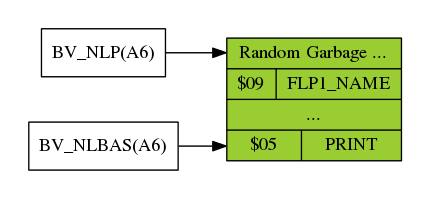
\includegraphics[width=0.5\textwidth]{Content/images/Name_List.png}
\caption{SuperBasic Name List Structure.}
\label{fig:SuperBasicNameListStructure}
\end{figure}

How is the name list useful to us in writing procedures and
    functions? consider these commands:

\begin{lstlisting}[firstnumber=1,]
OPEN_IN #3,'ram1_test_file'
OPEN_IN #3,ram1_test_file
\end{lstlisting}

What is the difference? In the first case, the parameter for the
    filename is a quoted string and internally, the OPEN\_IN routine can fetch
    it using \vector{CA\_GTSTR} as described above. In the second, it will fail if it
    uses \vector{CA\_GTSTR} because without quotes, the parameter is a NAME and not a
    STRING.

The procedure/function writer must check for a string parameter or a
    name parameter and treat each accordingly. How is this done? -{} use the
    name table type byte as described above.

In the procedure or function, process a name as follows:

Assuming that A3 points to the name table entry for this parameter,
    then if bits 0 to 4 of 1(a6,a3.l) is zero then we have a name and not a
    variable. We must copy the bytes of name, from the entry in the name list, to the stack (or to the appropriate buffer) making sure that the size byte in the name list is converted to a
    size word on the stack or in the buffer. The following fragment of code
    gives the general idea:

\begin{lstlisting}[firstnumber=1,]
name_test   move.b  1(a6,a3.l),d0
            andi.b  #$0f,d0
            bne.s   not_name
got_name    ;
            ; Must be a name so process accordingly here
            ;
not_name    ; Process a string here
\end{lstlisting}

So when a name is detected we have to make space for it, copy the
    size \emph{byte} from from the name list into the size \emph{word} in our string buffer
    (which has to be word aligned on an even address) and then copy the
    individual bytes from the name list to the string buffer. At this point we
    are in the same situation we would be in had we fetched a string using
    \vector{CA\_GTSTR} and copied it from the maths stack into our buffer. Simple? (In
    my famous DJToolkit\program{DJToolkit} extensions I never actually bothered doing this and I
    simply fetched all filenames etc as strings -{} if the user supplied a name
    instead, the procedure or function complained. So far no-{}one has
    requested that it be updated to allow names!)

\program{NLIST}\index{Printing the Name List}How about a bit of fun -{} lets write a procedure that prints the
    entire name list to a channel. It shall be called nlist and it shall take
    one parameter which is the channel number -{} this will default to \#1 if no
    parameter supplied.

\begin{lstlisting}[firstnumber=1,caption={Procedure to Print the Entire Name List},label={lst:NlistProcedure}]
bv_nlbas    equ     $20             ; Base of name list
bv_nlp      equ     $24             ; End of name list
bv_chbas    equ     $30             ; Base of channel table
bv_chp      equ     $34             ; End of channel table
err_no      equ     -6              ; Channel not open error
err_bp      equ     -15             ; Bad parameter error

start       lea     define,a1       ; Pointer to the definitions
            move.w  BP_INIT,a2      ; The vector we need to use
            jsr     (a2)            ; Call the vectored routine
            rts                     ; Return to SuperBasic

*----------------------------------------------------------------
* Definition table for one new procedure
*----------------------------------------------------------------
define      dc.w    1               ; 1 new procedure
            dc.w    nlist-*         ; Offset to procedure
            dc.b    5,'NLIST'       ; Size and name
            dc.w    0               ; End of procedures

            dc.w    0               ; Number of functions
            dc.w    0               ; End of functions

*----------------------------------------------------------------
* Procedure NLIST starts here ...
*
* Check for one or zero parameters - if not then error exit
*----------------------------------------------------------------
nlist       cmpa.l  a3,a5           ; No parameters?
            beq.s   nl_none         ; Yes, skip
            move.l  a5,d0           ; Last parameter pointer
            sub.l   a3,d0           ; minus first
            cmpi.w  #8,d0           ; One parameter?
            beq.s   got_one         ; Yes

bad_par     moveq   #-15,d0
error_exit  rts

*----------------------------------------------------------------
* If one parameter, must have a hash else error exit
*----------------------------------------------------------------
got_one     btst    #7,1(a6,a3.l)   ; check for a hash
            beq.s   bad_par         ; Not got one

*----------------------------------------------------------------
* It has a hash - fetch the channel id. If this fails, error exit.
*----------------------------------------------------------------
get_one     move.w  ca_gtint,a2     ; Vector for word integers
            jsr     (a2)            ; Fetch!
            tst.l   d0              ; Ok?
            bne.s   error_exit      ; No, bale out
            cmpi.w  #1,d3           ; One only?
            bne.s   error_exit      ; No, bale out
            move.w  0(a6,a1.l),d0   ; Fetch channel number
            addq.l  #2,a1           ; Tidy stack
            tst.w   d0              ; Set flags
            blt.s   bad_par         ; Negative is a bad id
            bra.s   chan_ok         ; skip default handling

*----------------------------------------------------------------
* No parameters supplied - default channel number to #1
*----------------------------------------------------------------
nl_none     moveq   #1,d0           ; Default to channel #1
chan_ok     bsr.s   channel_id      ; convert to channel id in A0
            bne.s   error_exit      ; Oops!

*----------------------------------------------------------------
* Fetch the start of the name list from BV_NLBAS(A6). The result 
* of this is an offset from A6 to where the namelist actually 
* starts.
*----------------------------------------------------------------
            move.l  bv_nlbas(a6),a3 ; Start of name list 
*                                   ; Relative to A6!

*----------------------------------------------------------------
* Our main loop starts here. We test to see if we are finished 
* and if not copy the (next) name to the buffer formatting it as 
* a QDOS string. 
* D3 is preserved inside the loop, so set it once just before the 
* loop starts.
*----------------------------------------------------------------
            moveq   #-1,d3          ; Timeout for the channel

nl_loop     cmpa.l  bv_nlp(a6),a3   ; Compare offsets - done?
            bge.s   nl_done         ; Yes
            moveq   #io_sstrg,d0    ; Print some bytes please
            move.b  0(a6,a3.l),d2   ; Counter byte from name list
            ext.w   d2              ; Needs to be word sized
            lea     1(a6,a3.l),a1   ; Start of bytes to print
            adda.w  d2,a3           ; Adjust to end of bytes
            addq.l  #1,a3           ; A3 = next entry, size byte
            trap    #3              ; Print the name 
*                                   ; Preserves A0, A3 and D3
            tst.l   d0              ; Ok?
            bne.s   error_exit      ; Oops - failed

nl_nl       moveq   #io_sbyte,d0    ; Code for 'send one byte'
            moveq   #10,d1          ; Newline character
            trap    #3              ; Print newline
*                                   ; Preserves A0, A3 and D3
            tst.l   d0              ; Ok?
            bne.s   error_exit      ; Oops - failed

            bra.s   nl_loop         ; Lets go round again!

*----------------------------------------------------------------
* If there is no more to do, return to SuperBasic.
*----------------------------------------------------------------
nl_done     moveq   #0,d0           ; No errors
            rts                     ; Exit to SuperBasic

*----------------------------------------------------------------
* Copy the above code for the CHANNEL_ID subroutine to here as it
* is required.
*----------------------------------------------------------------
channel_id ...
\end{lstlisting}

Save the file, assemble, fix typing errors and test -{} super stuff
    this eh?

When this procedure runs, you can see all the internal names like
    PRINT, CLOSE etc and also all your own stuff like NLIST, GREEN, RED etc
    and also any filenames that you have used without quotes around them.
    These are names like anything else.

if you try the following:

\begin{lstlisting}[firstnumber=1,]
open_new #3,ram1_test
nlist #3
close #3
\end{lstlisting}

then load ram1\_test into your editor (or copy to scr\_), the last
    entry in the name list will be ram1\_test -{} because you didn't use quotes.
    If you now try:

\begin{lstlisting}[firstnumber=1,]
open_new #3,"ram1_test_again"
nlist #3
close #3
\end{lstlisting}

This time, ram1\_test\_again will NOT be in the list because it is not
    a name, simply a string. This routine can be used to get a list of all
    procedures, functions, names etc that are loaded into your QL.

\section{The Maths Stack}\index{Maths Stack}
\label{ch7-maths-stack}%\hyperlabel{ch7-maths-stack}%

The maths stack is where all internal mathematical calculations of
    floating point variables are done. It is also used to allow parameters
    passed to machine code procedures and functions to be `collected' from the
    user and passed to the registers etc for use by the procedure or
    function.

The maths stack is simply an area of memory which can be used for
    all these fancy calculations, parameter handling etc. There is nothing
    (much) special about it and it is \emph{always} addressed internally using
    register A1 (relative to A6 -{} but you knew that didn't you?)

One of the first things I learned when writing extensions to
    SuperBasic was that on entry to a function or procedure, the A1 register
    is set to a value corresponding to the top of the maths stack. This is a
    \emph{myth} and is not correct.

The value in register A1 can be anything on entry to a machine code
    function or procedure. I have done a lot of investigating (thanks to
    QMON2\program{QMON2}) and come up with the following rule:

If you want a suitable value in A1 for the top of the maths stack,
    then either fetch some parameters, or, load it from BV\_RIP.

This means that if a function wants to return a value -{} which
    functions usually do -{} and the function has no parameters then you must
    load A1 from BV\_RIP(A6) before calling the \vector{BV\_CHRIX} vector to reserve
    space. As I found out to my cost, not setting A1 is a good way to trash
    the system!

If your function does have parameters, then AFTER they have been
    fetched, A1 is set ok, up until that time, it is not and has the following
    possible values:

\subsection{A1 Is Negative}
\label{ch7-A1-negative}%\hyperlabel{ch7-A1-negative}%

If A1 is a negative number, then your function has been called as
      part of an expression such as:

\begin{lstlisting}[firstnumber=1,]
PRINT 10 * MY_FUNCTION(p1, p2, p3 ....)
\end{lstlisting}

The number in A1.L is the number of bytes that have already been
      used on the maths stack for the `10' in this case. This will be -{}6 as
      the 10 will be stored as a floating point number.

\subsection{A1 Is Zero}
\label{ch7-A1-zero}%\hyperlabel{ch7-A1-zero}%

If the number in A1 is zero, then your function has been called
      thus:

\begin{lstlisting}[firstnumber=1,]
PRINT MY_FUNCTION(p1, p2, p3 ....)
\end{lstlisting}

or

\begin{lstlisting}[firstnumber=1,]
PRINT MY_FUNCTION(p1, p2, p3 ....) + 10
\end{lstlisting}

and no bytes have been used on the maths stack yet.

\subsection{A1 Is Positive}
\label{ch7-A1-positive}%\hyperlabel{ch7-A1-positive}%

If A1.L is greater than zero then this implies that there are A1.L
      many bytes available on the maths stack and calling \vector{BV\_CHRIX} to allocate
      stack space will not move the maths stack around in memory.

\begin{warning}
I have \emph{never} seen this documented and it
        has been discovered by me during long debugging sessions. Now that
        SMSQ is here, the above information may no longer be valid. The
 \emph{only} thing to remember is that on entry to a
        procedure or function, A1 \emph{does not} hold a
        suitable value for the top of the maths stack as stated in various
        documents.
\end{warning}

So that is the real situation and not as specified in the
      documentation. I took ages to debug one simple function I wrote, which
      had no parameters and required some space on the maths stack for its
      result. Take a look at the code in the colour functions (green, red etc)
      we wrote back at the start of this article and you will see the
      following code:

\begin{lstlisting}[firstnumber=1,]
return_d7   move.l  bv_rip(a6),a1   ; Because we had no params
            moveq   #2,d1           ; Size of stack space needed
            move.w  bv_chrix,a2     ; Allocate maths stack space
            jsr     (a2)            ; Get some space
\end{lstlisting}

As you can now see, we load A1 from BV\_RIP because none of the
      functions had any parameters passed. Had that one line of code been
      missed out, your QL would have crashed. Try it if you like!

Values on the maths stack must be stored at even addresses. For
      integers, long integers and floating point values, this is not a
      problem. Strings, on the other hand, must be set up correctly with the
      word defining the size n an even address and the bytes of the string
      following. Odd length strings should have an extra padding byte to keep
      the A1 maths stack pointer even.

If you read back to section ~\ref{ch7-keep-things-even} `Keeping things
      even' then you will see how to do this. If you are returning a string
      from a function, you will need to reserve space for the string, its
      word count and a possible spare byte for padding. Refer to the
      explanation above and you will see why the following code `just works'
     :

\begin{lstlisting}[firstnumber=1,]
ret_string  move.w  (a0),d1         ; Assume string is at (A0)
            addq.w  #3,d1           ; Add size word + padding
            bclr    #0,d1           ; Force even size
            move.w  bv_chrix,a2     ; Allocate maths stack space
            jsr     (a2)
\end{lstlisting}

Of course, I am assuming that A1 holds a suitable value. The code
      above will request an even amount of space for a string result. First we
      fetch the length into D1 -{} this is the number of characters in the
      string only.

We then add 3 to D1. This is 2 for the word count and one for a
      possible padding byte. By clearing bit zero of D1 we force the number to
      be even and can then carry on with the request for space etc. Easy stuff
      this!

\section{Returning Values From Functions}\index{Function Return Values}
\label{ch7-returning-values}%\hyperlabel{ch7-returning-values}%

When returning values on the maths stack you must be very careful.
    When a function exits there must be a value on the top of the maths stack
    the pointer to this value needs to be stored in BV\_RIP(A6) and D4 has to
    have a values in it which defines the returned parameter type. See Table ~\ref{tab:FunctionReturnDataTypes}.

\begin{table}[htbp]
\centering
\begin{tabular}{l l}  % Set this correctly ...
\toprule
\textbf{D4} & \textbf{Return Parameter Type} \\
\midrule
%
1 & String\\
2 & Floating point\\
3 & Word integer\\%
\bottomrule
\end{tabular}
\caption{Function Return Data Types}
\label{tab:FunctionReturnDataTypes}
\end{table}

Notice anything missing? Although we are allowed to fetch long
    integers as parameters, we are not allowed to return them. This is a
    problem and the usual fix is to convert a long integer to a floating point
    and return that instead. This will be covered in another thrilling episode
   !

\section{Channel Tables}\index{SuperBasic Channel Table}
\label{ch7-channel-table}%\hyperlabel{ch7-channel-table}%

In our procedure PSI\_CLS\program{PSI\_CLS}, we use a channel number in SuperBasic. In
    assembler, this is no use to us as all internal operations that require a
    channel (CLS, PAPER etc) require a channel id which is a 32 bit long
    number which bears no resemblance (or only coincidentally) to a SuperBasic
    channel number.

In QDOS there is a channel table -{} for the entire system, and there
    is the SuperBasic channel table which is used to convert channel numbers
    into channel ids which is what we require. SuperBasic keeps us away from
    nasty things like internal representations -{} assembler does not.

The routine we used above, channel\_id, is all that is required to
    convert a channel number to a channel id. It looks at the SuperBasic
    channel table and for each channel that has been opened (even if it is now
    closed) there will be an entry in the channel table. Each entry is \$28
    bytes long (40 bytes) and has the structure shown in Table ~\ref{tab:SuperBasicChannelTableDefinition}.

\begin{table}[htbp]
\centering
\begin{tabular}{l l p{0.75\linewidth}}  % Set this correctly ...
\toprule
\textbf{Offset} & \textbf{Size} & \textbf{Purpose} \\
\midrule
%
\$00 & Long    & QDOS internal channel id\\
\$04 & 6 bytes & Graphics cursor X position (Floating Point format)\\
\$0A & 6 bytes & Graphics cursor Y position (Floating Point format)\\
\$10 & 6 bytes & Turtle angle (Floating Point format)\\
\$16 & Byte    & Pen status (0 = up or 1 = down)\\
\$20 & Word    & Character position on line for PRINT and INPUT etc\\
\$22 & Word    & Width of the channel. Set by WIDTH command in SuperBasic but defaults to 80 when OPEN is called.\\
\$24 & Long    & Spare -{} currently unused\\
%
\bottomrule
\end{tabular}
\caption{SuperBasic Channel Table Definition}
\label{tab:SuperBasicChannelTableDefinition}
\end{table}


When a channel is opened in SuperBasic, an entry is created (or
    reused) in this table. At startup channels \#0, \#1, and \#2 are pre-{}created
    and that is all. If you now open \#4, a new entry will be created for it.
    If you open channel \#10, then blank entries are created for all the
    `in-{}between' channels (5 to 9) and entry 10 is then created and
    initialised on top.

A channel that has never been opened can therefore still have an
    entry in this table -{} channels 5 to 9 in the above example. All of these
    use memory so it is advisable to start with 3 and work upwards opening
    channels as you go, rather than opening \#100 or something similar which
    needlessly wastes 40 bytes of memory for each unused channel.

A channel that is closed, or has never been opened, has a QDOS
    channel id which is negative.

In the Basic variables area in QDOS (to be covered in a later issue
    -{} and by the way, I refer to the variables that hold information about
    SuperBasic, and not variables you create in SuperBasic!) BV\_CHBAS holds
    the offset from A6 to the first entry in the table (ie channel \#0) and
    BV\_CHP holds the offset from A6 to the first byte after the last entry in
    the channel table. Don't forget that these are offsets and that everything
    in SuperBasic is relative to A6 -{} simply because by doing this the base
    address for the job (SuperBasic is just another job in the machine) is
    held in A6. If everything else is stored as an offset then moving the job
    in memory is simple as only the A6 register has to be updated.

Take a look at the code for channel\_id again and note how we are
    using addresses that are relative to A6. Make sure that you understand
    because all fiddling in the bowels of SuperBasic requires that you
    understand relative addressing.

Most of the time you will only be interested in the conversion from
    SuperBasic channel number to QDOS channel id.

\section{Exercise}
\label{ch7-exercise}%\hyperlabel{ch7-exercise}%

As an exercise, why not add a new procedure called \program{PSI}PSI to the code
    for PSI\_CLS.\program{PSI\_CLS} This new procedure will carry out all the same work as
    PSI\_CLS but it will not do the CLS part of it. This will be useful when
    you want to set the colours for a window but not clear it. I will NOT be
    giving the answers out next time, but here are a few hints:
\begin{itemize}[itemsep=0pt]

\item{}update the definition table with details of the new
        procedure.


\item{}in the proc's code, set D6.B to zero for PSI and 1 for PSI\_CLS.
        Do this as the first instruction in both procedures.


\item{}In the PSI procedure, simply set D6 and jump to the code in
        PSI\_CLS.


\item{}Just before doing the actual CLS part of PSI\_CLS, check the
        value in D6.B and if zero, don't do the CLS simply BRA.S to error\_exit
        instead.

\end{itemize}

All in all, I think this can be done in about 10 extra lines of
    code, maybe less, not counting the extra lines in the definition
    block.

\begin{warning}
Adding even a few lines of code can sometimes cause any `short'
      branches to go out of range and this will cause errors in the assembly.
      If this happens, simply find the ones in error and remove the `.s' from
      the `bsr' or `bra' instructions.
\end{warning}

\section{Coming Up...}
\label{ch7-the-end}%\hyperlabel{ch7-the-end}%

In the next chapter we delve into the QL's screen layout and using
    our new found knowlege of assembly language programming, we will develop a
    mode 4 `plot' routine in assembler. If you find this easy, there is an
    exercise for the reader -{} to develop the corresponding mode 8 `plot' code
   !

